%
% Documento: FRAMEWORK PROPOSTO
%
\chapter{Módulos}\label{chap:imp}
    O framework consiste em alguns módulos básicos, cada um com suas devidas utilidades e funções.
    A separação dos de cada módulos foi dada com base em suas caracteristicas e funcionalidades,

    \begin{figure}[H]
        \vspace*{0,3cm}
        \centering
        \caption{Diagrama de Componentes}
        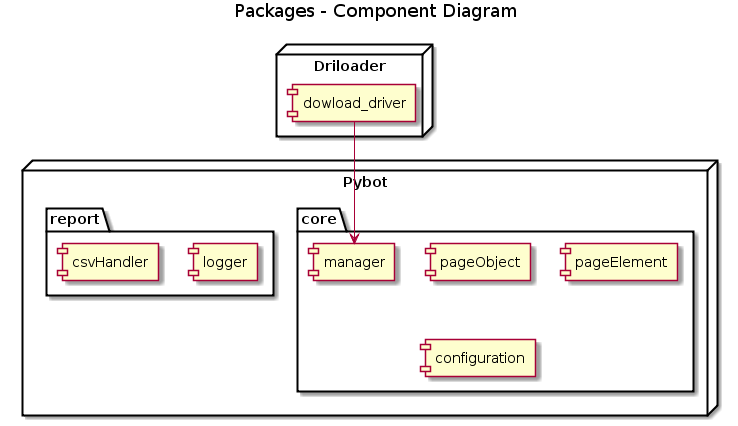
\includegraphics[width=1\textwidth]{./04-figuras/model}
        \label{fig:modules}
    \end{figure}

    \section{Core}
        Este módulo contém as funcionalidades básicas para a operação do framework com o Selenium \emph{Webdriver}
        e o gerenciamento dos parâmetros de execuções de cada script.

        \subsection{Manager}
        Manager server para abstrair o uso do Selenium \emph{Webdriver} criando uma camada de metodos própios fazendo com que caso alguma
        atualização da API do Selenium \emph{Webdriver} altere os \emph{scripts} criados não sejam impactados. Fazendo uso do Driloader mencionado na
        subseção \ref{driloader} ele verifica a necessidade do download do driver para poder executar o \emph{Selenium Webdriver}.

        \subsection{Configuration}
        Responsável por gerar as configurações básicas para o framework e disponibilizá-las no arquivo \emph{pybot.ini}.
        Este arquivo é criado para cada script do usuário e nele arquivo é possível adicionar qualquer tipo de configurações ou parâmetros
        necessárias para o usuário, apenas sendo preciso seguir os padrões descrito na imagem \ref{fig:pybot.ini} e utilizando com o comando
        \mbox{\emph{configuration.getConfig('Seção', 'variável')}}

        \begin{figure}[H]
            \vspace*{0,3cm}
            \centering
            \caption{Estrutura pybot.ini}
            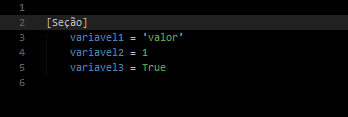
\includegraphics[width=0.7\textwidth]{./04-figuras/ini}
            \label{fig:pybot.ini}
        \end{figure}

    \section{Component}
    \label{Comp}
        Módulo criado para seguir os padrões de \emph{PageObject} e \emph{PageElement}, contendo abstração para os tipos de inputs do \emph{html}.

        \subsection{WebElement}
            Serve para abstrair o uso da classe WebElement do próprio Selenium Webdriver. Contendo uma classe para cada tipo de campo dos \emph{html},
            ele dispõe de algumas funcionalidades básica, como a atribuição de uma valor para um elemento do tipo \emph{input text} irá escrever
            valor dentro do campo, \emph{select} irá selecionar a opção cujo texto seja igual ao valor informado, \emph{radio} irá selecionar o
            a opção que tenha o \emph{value} do valor informado e para o tipo \emph{checkbox} irá marcar ou desmarcar as opções se o valor for
            verdadeiro(True) ou falso(False)

        \subsection{PageElement e PageElements}
        \label{PageElement}
            Essas classes servem para controlar os elementos mapeados das telas. Sempre quando serão acessadas a classe faz novamente a pesquisa
            do elemento em tela, prevenindo assim uma das exceções mais comum do Selenium Webdriver que é a \emph{StaleElementReferenceException},
            que é quando o elemento em questão não existe mais no DOM ou a referência que tinha não é mais a mesma. Conta com uma lista de seletores
            que facilitam para o usuário buscar os elementos e deixam o código mais legível. Usa-se a classe PageElements quando quiser pegar mais
            de um elemento com o mesmo seletor.

            \begin{figure}[H]
                \vspace*{0,3cm}
                \centering
                \caption{Lista de Seletores}
                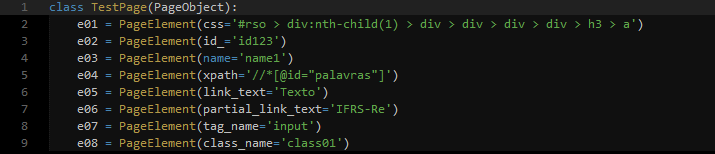
\includegraphics[width=1\textwidth]{./04-figuras/selectors}
                \label{fig:selectors.png}
            \end{figure}

        \subsection{PageObject}
            Classe simbolica, serve apenas para poder juntar diversos PageElement descritos pelo usuário em uma classe para melhor
            legibilidade e componentização das páginas mapeadas.

    \section{Report}

        Estes módulo está destinado para geração de logs de execuções internas do framework, criação e controle
        de logs definidos pelos usuário e a criação de planilhas analíticas de dados extraídos das páginas.

        \subsection{Logger}
        Classe de geração dos Logs de execução do framework.

        \subsection{CsvHandler}
        Utilizado para geração de planilhas com dados extraídos das páginas para análise posterior do usuário.

    \section{Driloader}
    \label{driloader}
        Driloader é o responsável pelo download dos \textit{drivers} de cada \emph{browser},suportando \textit{download} dos \textit{drivers} do Internet Explorer,
        Firefox e Chrome, sendo possível para o usuário selecionar uma versão específica, a ultima versão ou detectar automaticamente qual a versão adequada para o \emph{browser} instalado do usuário. Como para utilização do Selenium
        Webdriver é necessário um \textit{driver} específico de cada \emph{browser} foi tomada a decisão da criação desse projeto,
        inicialmente o Driloader era um módulo do framework mas pela autonomia e praticidade que ele proporciona aos usuários do Selenium Webdriver foi feita a separação dele do Pybot.



